\chapter{Especificação de Requisitos} \label{cap:especificacao}

%%%%%%%%%%%%%%%%%%%%%%%%%%%%%%%%%%%%%%%%%%%%%%%%%%%%
%%%%%%%%%%%%%%%%%%%%%%%%%%%%%%%%%%%%%%%%%%%%%%%%%%%%

\section{Especificação da arquitetura do sistema}
\label{sec:requisitos_infra}

A arquitetura especificada neste trabalho define a organização técnica da solução proposta para comunicação, encaminhamento e persistência dos dados produzidos na rede de campo. Sua função é estruturar, de forma coerente, os componentes responsáveis pela coleta das informações, pela transição entre a comunicação embarcada e a infraestrutura de aplicação, e pelo armazenamento dos dados necessários ao funcionamento do sistema e às etapas posteriores de segurança e análise.

A solução foi organizada em quatro blocos principais: nó sensor, \textit{gateway}, \textit{backend} com API e persistência. No trecho de campo, o nó coleta os dados do ambiente e transmite quadros curtos por um enlace LoRa ponto a ponto, atendendo aos requisitos de operação em dispositivos com restrição energética. O \textit{gateway} concentra em um único dispositivo os papéis que o modelo LoRaWAN distribui entre \textit{gateway}, \textit{network server} e \textit{application server}: recebe os quadros, verifica a autenticidade e a ordem, registra os metadados de recepção e encaminha as mensagens ao \textit{backend}, em conformidade com os requisitos RF3, RF6 e RF12.

A partir do \textit{gateway}, a comunicação passa a utilizar Wi-Fi e requisições HTTP, integrando a rede embarcada a uma API autenticada e a um mecanismo centralizado de persistência, implantados em infraestrutura local, na mesma rede do \textit{gateway}. Essa escolha mantém a coleta independente de conectividade externa e dispensa a negociação de certificados no dispositivo embarcado; a migração para infraestrutura em nuvem, com transporte cifrado, é tratada como extensão e discutida no Capítulo~\ref{cap:consideracoes}. A camada de aplicação permanece disponível de forma contínua para o recebimento dos dados encaminhados pelo \textit{gateway}, e o próprio \textit{gateway} mantém os quadros em memória quando a API está indisponível.

Além dos dados de aplicação, como temperatura e luminosidade, a arquitetura prevê a persistência de metadados relevantes para o acompanhamento da comunicação, incluindo informações de origem, sequência, recepção e qualidade do enlace. Essa escolha atende aos requisitos RF5 e RF7 e contribui para a rastreabilidade da operação, conforme estabelecido em RNF6. Cada registro carrega ainda o identificador da sessão em que foi recebido e a indicação de ter sido entregue em tempo real ou reenviado após uma falha de conectividade (RF9 e RF10), de modo que uma queda da rede entre \textit{gateway} e \textit{backend} nunca se confunda com perda no enlace de rádio. A mesma base persistida prepara a infraestrutura para a incorporação de mecanismos de criptografia leve e de análise por aprendizado de máquina, em conformidade com RNF7 e RNF8.

A Figura~\ref{fig:arquitetura-especificada} apresenta a arquitetura técnica especificada para o sistema. A partir dessa organização, as subseções seguintes detalham os requisitos funcionais e não funcionais da infraestrutura proposta, que fundamentam e justificam as decisões arquiteturais adotadas.

\begin{figure}[htb]
  \caption{\label{fig:arquitetura-especificada}Arquitetura especificada do sistema proposto.}
  \begin{center}
      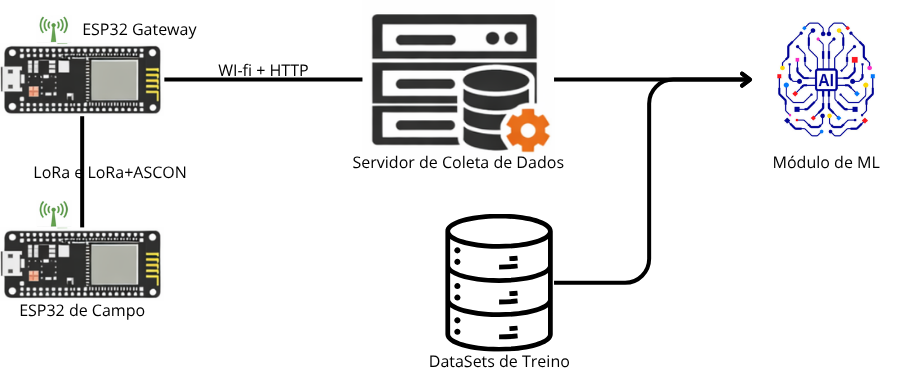
\includegraphics[scale=0.5]{figuras/arch_figure1.png}
  \end{center}

\end{figure}

%%%%%%%%%%%%%%%%%%%%%%%%%%%%%%%%%%%%%%%%%%%%%%%%%%%%

\subsection{Requisitos funcionais da infraestrutura proposta}

Os requisitos funcionais da infraestrutura proposta descrevem os comportamentos esperados da arquitetura do sistema, considerando a coleta, o encaminhamento, a autenticação e a persistência das informações produzidas na rede de campo.

\begin{enumerate}
    \item[RF1.] O sistema deve permitir que os nós de campo coletem e transmitam dados de aplicação, incluindo, no protótipo previsto, informações de temperatura e luminosidade.

    \item[RF2.] Cada mensagem transmitida pelos nós deve conter, além dos dados de aplicação, informações mínimas de identificação e acompanhamento, incluindo identificador do dispositivo e contador de mensagens.

    \item[RF3.] O gateway deve receber as mensagens provenientes da rede de campo, registrar os metadados de recepção e encaminhar essas informações ao backend por meio de rede Wi-Fi e requisições HTTP.

    \item[RF4.] O backend deve autenticar as requisições enviadas pelo gateway, restringindo o recebimento de dados a dispositivos previamente autorizados.

    \item[RF5.] O sistema deve persistir os dados de aplicação recebidos dos nós juntamente com os metadados associados à comunicação.

    \item[RF6.] A infraestrutura deve permitir armazenamento temporário das mensagens no gateway em situações de indisponibilidade da conexão com o backend, com possibilidade de reenvio posterior.

    \item[RF7.] Os dados persistidos devem permanecer disponíveis para uso posterior pelas camadas de segurança e de análise por aprendizado de máquina.

    \item[RF8.] O gateway deve registrar cada quadro recebido em sua interface serial, em formato legível por máquina, independentemente do estado da conexão com o backend, de modo que a coleta nunca dependa da rede.

    \item[RF9.] O sistema deve identificar sessões de operação, de modo que quadros recebidos após um reinício do nó ou do gateway não sejam confundidos com a continuação da sequência anterior.

    \item[RF10.] Cada quadro persistido deve indicar sua origem: entregue em tempo real, reenviado a partir do armazenamento temporário do gateway ou relido de um registro serial.

    \item[RF11.] O gateway deve emitir periodicamente um sinal de vida com contadores de quadros recebidos, rejeitados e encaminhados, para distinguir ausência de tráfego de falha do próprio gateway.

    \item[RF12.] O gateway deve descartar, sem encaminhar, quadros com tamanho diferente do esperado, com falha de verificação de integridade, com falha de autenticação ou com contador não crescente, contabilizando cada caso separadamente.

\end{enumerate}

%%%%%%%%%%%%%%%%%%%%%%%%%%%%%%%%%%%%%%%%%%%%%%%%%%%%

\subsection{Requisitos não funcionais da infraestrutura proposta}

Os requisitos não funcionais da infraestrutura proposta descrevem propriedades de operação e restrições que devem ser observadas para que a solução seja compatível com o contexto de sistemas embarcados e Internet das Coisas. Para sua elicitação e organização, adotou-se como referência a norma ISO/IEC 25010, considerando principalmente características relacionadas à eficiência de desempenho, confiabilidade, compatibilidade, manutenibilidade e segurança.

\begin{enumerate}
    \item[RNF1.] A infraestrutura deve ser compatível com a operação de nós de campo com restrições de energia, priorizando baixo consumo no trecho embarcado da comunicação.

    \item[RNF2.] A comunicação do sistema deve ser orientada a evento, evitando transmissões contínuas desnecessárias entre os componentes.

    \item[RNF3.] A arquitetura deve manter separação clara entre a rede de campo, baseada em LoRa ponto a ponto, e a infraestrutura de aplicação, baseada em Wi-Fi e HTTP, de modo que a recepção de rádio nunca aguarde a rede.

    \item[RNF4.] O protótipo deve preservar simplicidade de integração entre hardware, comunicação e backend, de modo a manter viável sua montagem e evolução no contexto do projeto.

    \item[RNF5.] A infraestrutura deve apresentar robustez básica a falhas temporárias de conectividade entre gateway e backend.

    \item[RNF6.] O sistema deve garantir rastreabilidade das mensagens recebidas, por meio do registro de dados e metadados que permitam identificar origem, sequência, instante de recepção e condições básicas do enlace.

    \item[RNF7.] A arquitetura deve ser compatível com a incorporação posterior de mecanismos de criptografia leve sem exigir reformulação completa da infraestrutura de comunicação.

    \item[RNF8.] A infraestrutura deve ser compatível com o uso posterior de técnicas de aprendizado de máquina aplicadas à análise do comportamento da rede e à detecção de anomalias.
    
    \item[RNF9.] O quadro transmitido não deve exceder 51 bytes, limite do plano regional AU915 na taxa de dados mais lenta, de modo que possa ser transmitido em qualquer fator de espalhamento.

    \item[RNF10.] Os metadados de recepção registrados devem ter os mesmos campos e a mesma semântica das variáveis candidatas dos modelos de detecção, permitindo comparar a coleta própria com o conjunto de dados de referência sem transformação adicional.

    \item[RNF11.] O envio ao backend não deve bloquear a recepção de rádio: um quadro que chegue durante uma requisição HTTP em andamento deve ser recebido e registrado normalmente.

\end{enumerate}

%%%%%%%%%%%%%%%%%%%%%%%%%%%%%%%%%%%%%%%%%%%%%%%%%%%%

\subsection{Rastreabilidade dos requisitos da infraestrutura}
\label{subsec:rastreabilidade_infra}

A Tabela~\ref{tab:rastreabilidade_infra} relaciona cada requisito ao componente que o atende e à forma como foi verificado. Os detalhes de implementação estão no Capítulo~\ref{cap:desenvolvimento}. Três requisitos estão atendidos apenas em parte e são declarados como tal: o RF1, porque os dados de aplicação ainda são sintéticos; o RF6, cuja lógica foi testada mas cujo reenvio não foi exercitado em uma queda real de rede; e o RNF1, porque o nó ainda não entra em modo de baixo consumo entre transmissões.

\begin{table}[htb]
\centering
\caption{Rastreabilidade dos requisitos da infraestrutura}
\label{tab:rastreabilidade_infra}
\small
\begin{tabular}{lp{5,8cm}p{6,2cm}}
\hline
\textbf{Req.} & \textbf{Onde é atendido} & \textbf{Como foi verificado} \\
\hline
RF1  & Firmware do nó; 4 bytes de dados no quadro & Coletas de 23/08 e 24/09; dados sintéticos (parcial) \\
RF2  & Cabeçalho do quadro: identificador e contador & Teste na placa do quadro; coletas \\
RF3  & Gateway: recepção no núcleo 1, envio HTTP no núcleo 0 & 857 quadros entregues em 24/09 \\
RF4  & Token no cabeçalho HTTP, comparação em tempo constante & Testes automatizados do backend \\
RF5  & Banco SQLite com os 12 campos e metadados de ingestão & Testes; conferência serial contra banco \\
RF6  & Fila e armazenamento temporário de 512 registros no gateway & Lógica testada na placa; não exercitado em campo (parcial) \\
RF7  & API de consulta e exportação em CSV & Ferramenta de análise; notebooks \\
RF8  & Registro serial sob exclusão mútua, anterior ao envio & Coleta de 23/08 sem backend \\
RF9  & Identificador de sessão: sorteio na inicialização mais contador de sessão & Teste na placa; sessão única em 24/09 \\
RF10 & Campo de origem por idade do registro na entrega & 857 quadros marcados como tempo real \\
RF11 & Sinal de vida a cada 30 s na serial e na API & Registro serial; envio à API pendente de gravação \\
RF12 & Verificação de tamanho, CRC, janela anti-replay e tag & Teste na placa: quadro forjado não avança a janela \\
RNF1 & Potência de 5 dBm; nó sem modo de repouso & Parcial: repouso entre transmissões pendente \\
RNF2 & Recepção por interrupção; transmissão periódica & Coletas \\
RNF3 & Dois núcleos com fila de espera zero & 0 perdas em 857 quadros com backend ativo \\
RNF4 & Contrato único compartilhado pelos dois firmwares & Compilação; testes \\
RNF5 & Armazenamento temporário e espera exponencial de 1 a 30 s & Lógica testada na placa \\
RNF6 & 12 campos mais identificadores de gateway, sessão e instante UTC & Conferência serial contra banco \\
RNF7 & Adaptador de cifra com seleção em tempo de compilação & AES-GCM no ar; Ascon pendente \\
RNF8 & Mesmos campos das variáveis candidatas dos modelos & Análise das coletas \\
RNF9 & Quadro de 26 bytes; verificação em tempo de compilação & Compilação \\
RNF10 & Formatação byte a byte do registro & Teste na placa \\
RNF11 & Fila entre núcleos com espera zero & 0 perdas com backend ativo \\
\hline
\end{tabular}
\legend{Fonte: elaborado pelos autores (2026).}
\end{table}


%%%%%%%%%%%%%%%%%%%%%%%%%%%%%%%%%%%%%%%%%%%%%%%%%%%%
%%%%%%%%%%%%%%%%%%%%%%%%%%%%%%%%%%%%%%%%%%%%%%%%%%%%

\section{Requisitos do Sistema de Detecção de Anomalias}
A incorporação de um modelo de aprendizado de máquina à arquitetura proposta 
introduz requisitos específicos, distintos dos requisitos de infraestrutura 
definidos na Seção~\ref{sec:requisitos_infra}. O modelo será treinado e 
avaliado em ambiente computacional convencional, utilizando os dados 
históricos do \textit{dataset} Tour Perret. A viabilidade de portabilidade 
da fase de inferência para o gateway é tratada como perspectiva de 
continuidade, conforme discutido na Seção~7.3.

%%%%%%%%%%%%%%%%%%%%%%%%%%%%%%%%%%%%%%%%%%%%%%%%%%%%

\subsection{Requisitos Funcionais}

\begin{enumerate}

    \item[RF1.] O sistema deve receber como entrada sequências temporais das 
    variáveis selecionadas, organizadas por dispositivo e ordenadas 
    cronologicamente.

    \item[RF2.] O sistema deve produzir previsões do comportamento esperado de 
    cada variável monitorada e calcular o resíduo entre valor previsto e 
    valor observado para cada instante de tempo.

    \item[RF3.] O sistema deve classificar cada observação como normal ou 
    potencialmente anômala, com base em um critério de limiarização definido 
    a partir do conjunto de validação.

    \item[RF4.] O sistema deve permitir comparação quantitativa entre as três 
    abordagens de modelagem (ARIMA, RNN, LSTM) através de métricas 
    padronizadas de qualidade de previsão e detecção.

\end{enumerate}


%%%%%%%%%%%%%%%%%%%%%%%%%%%%%%%%%%%%%%%%%%%%%%%%%%%%

\subsection{Requisitos Não Funcionais}

\begin{enumerate}

    \item[RNF1.] O treinamento deve ser realizado exclusivamente sobre dados que 
    representem operação normal da rede, sem contaminação por observações 
    potencialmente anômalas.

    \item[RNF2.] O processo de treinamento e avaliação deve ser reprodutível, com 
    registro das sementes de inicialização, hiperparâmetros e critérios de 
    seleção de ordem utilizados em cada modelo.

\end{enumerate}

Essa orientação fortalece a coerência do trabalho como um todo. Em vez de separar artificialmente a fase de modelagem da fase de implantação, o desenvolvimento já considera que a utilidade prática dos modelos depende de um equilíbrio entre eficácia de detecção e viabilidade de execução em dispositivos restritos. Assim, a implementação proposta dialoga diretamente com a etapa posterior de avaliação energética e computacional.

Sob essa perspectiva, a comparação entre modelos não deverá considerar apenas métricas tradicionais de desempenho, mas também aspectos como simplicidade estrutural, custo computacional, volume de memória.

%%%%%%%%%%%%%%%%%%%%%%%%%%%%%%%%%%%%%%%%%%%%%%%%%%%%
%%%%%%%%%%%%%%%%%%%%%%%%%%%%%%%%%%%%%%%%%%%%%%%%%%%%

\section{Requisitos de Segurança do Sistema criptográfico}
\label{sec:requisitos_seguranca}
\subsection{Segurança do Ascon-AEAD128 e da variante Ascon-128a}
A camada criptográfica especificada nesta seção é adicional à proteção já oferecida pelo protocolo de comunicação. A especificação do LoRaWAN determina que a carga útil de aplicação seja cifrada fim a fim entre o dispositivo e o \textit{Application Server}, mas registra que a proteção de integridade não é fim a fim: o \textit{Network Server} pode alterar o conteúdo cifrado em trânsito, ainda que sem conseguir lê-lo, uma vez que detém a chave empregada no cálculo do código de integridade das mensagens. Por esse motivo, a própria norma recomenda que aplicações que exijam confidencialidade e integridade fim a fim empreguem soluções de segurança adicionais \cite{lorawan104}. É essa lacuna de integridade que a camada baseada em Ascon preenche neste trabalho.

Para o uso seguro da cifra, este trabalho adota os requisitos operacionais especificados pelo NIST para o Ascon-AEAD128 \cite{nist800232}. Embora a implementação utilizada corresponda à variante Ascon-128a (versão 1.2), esses requisitos são adotados de forma conservadora como limites aplicáveis, uma vez que ambas as versões compartilham a mesma taxa de processamento e a mesma estrutura de permutação, conforme a Tabela~\ref{tab:parametros_ascon}, enquanto suas diferenças introduzem apenas sobrecarga constante. O primeiro requisito trata da geração da chave criptográfica, que deve seguir os padrões descritos no documento SP 800-133r2 \cite{barker2020nist133}, no qual é estabelecida a seguinte operação:

\[
K = U \oplus V,
\]

em que $U$ é uma cadeia de bits extraída de um Gerador de Bits Aleatórios (RBG - \textit{Random Bit Generator}) aprovado, e $V$ consiste em uma sequência de bits gerada independentemente de $U$, podendo ser composta inteiramente por zeros.

As especificações para os geradores de bits aleatórios aprovados estão descritas no documento SP 800-90A \cite{barker2015nist90a}. Neste projeto, é utilizado um Gerador Determinístico de Bits Aleatórios (DRBG - \textit{Deterministic Random Bit Generator}) através do mecanismo CTR\_DRBG. Essa escolha justifica-se pelo fato de que a entropia bruta extraída diretamente do hardware pode conter vícios físicos, tornando indispensável um estágio secundário de tratamento e condicionamento algorítmico \cite{turan2018nist90b}. Dessa forma, a implementação fará uso da biblioteca nativa \textit{mbedTLS} do ESP32, que extrai a entropia verdadeira do periférico de hardware (TRNG) e a processa através do algoritmo CTR\_DRBG, garantindo uma saída perfeitamente balanceada para a geração da chave.

Com base nesses elementos, os requisitos de segurança do Ascon-AEAD128 podem ser organizados em requisitos funcionais e não funcionais.

\subsubsection{Requisitos funcionais}

\begin{enumerate}
    \item[RF1.] A implementação da biblioteca \textit{ascon-suite} deve ser validada previamente, conforme discutido na Seção \ref{subsec:validacao-ascon}.

    \item[RF2.] A geração da chave criptográfica deve seguir os padrões descritos no documento SP 800-133r2 \cite{barker2020nist133}, adotando a operação $K = U \oplus V$, e empregar um gerador de bits aleatórios aprovado com força de segurança de, no mínimo, 128 bits \cite{nist800232}.

    \item[RF3.] O sistema deve utilizar um Gerador Determinístico de Bits Aleatórios (DRBG - \textit{Deterministic Random Bit Generator}) através do mecanismo CTR\_DRBG para a geração de chaves criptográficas.

    \item[RF4.] A implementação deve fazer uso da biblioteca nativa \textit{mbedTLS} do ESP32 para extrair a entropia verdadeira do periférico de hardware (TRNG) e processá-la através do algoritmo CTR\_DRBG.

    \item[RF5.] A renovação da chave de um nó deve ser feita por novo provisionamento, onde descarta-se o estado criptográfico do dispositivo, gera-se nele uma chave nova, nas condições do RF2 ao RF4, e atualiza-se o registro correspondente no receptor. A chave nova deve ser gerada de forma independente da anterior, sem derivar dela nem ser transportada sob sua proteção, como exige o SP 800-133r2 para a substituição de chave comprometida \cite{barker2020nist133}. Como os gatilhos preventivos de renovação (RNF3 e RNF4) são inalcançáveis na operação prevista, conforme discutido ao final desta seção, a renovação é um procedimento de resposta a um incidente, e não de rotina.

    \item[RF6.] Cada nó sensor deve possuir uma chave criptográfica própria, gerada e provisionada individualmente, de modo que o comprometimento físico de um nó não exponha o tráfego dos demais. Como a exigência de unicidade do \textit{nonce} se aplica a uma mesma chave, essa separação também restringe o escopo dessa garantia a um único dispositivo \cite{nist800232}.

    \item[RF7.] A unicidade do \textit{nonce} exigida pelo RNF2 deve ser assegurada por um contador monotônico mantido em memória não volátil no próprio dispositivo, incrementado a cada operação de cifragem e persistido antes da transmissão da mensagem correspondente, de modo que uma interrupção de energia descarte valores em vez de repeti-los. Após uma reinicialização, a leitura do valor persistido deve preceder qualquer operação criptográfica. O contador não deve ser derivado de valores mantidos pela pilha de comunicação, para que a garantia de unicidade não dependa de decisões tomadas em outra camada.

    \item[RF8.] A camada criptográfica deve detectar e rejeitar qualquer alteração da mensagem em trânsito, seja no texto cifrado, nos dados associados ou na própria \textit{tag} de autenticação. Em caso de falha na verificação de integridade, a decifragem deve retornar erro sem entregar à aplicação qualquer fragmento de texto claro \cite{nist800232}. Este requisito responde à lacuna descrita no início desta seção. A norma do LoRaWAN admite que o \textit{Network Server} altere o conteúdo cifrado em trânsito, ainda que sem conseguir lê-lo \cite{lorawan104}, e é a verificação da \textit{tag} pelo destinatário final que torna essa alteração detectável.

    \item[RF9.] O receptor deve recusar mensagens cujo \textit{nonce} já tenha sido aceito, mantendo registro do maior valor recebido de cada dispositivo e descartando valores repetidos ou regressivos. O modo AEAD garante integridade, mas não frescor, um pacote válido retransmitido sem alteração é legítimo do ponto de vista criptográfico, e sua detecção depende de estado mantido no receptor. Este requisito complementa o RF7, que assegura a unicidade do \textit{nonce} na origem, estendendo a garantia ao destino.
\end{enumerate}

\subsubsection{Requisitos não funcionais}

\begin{enumerate}
    \item[RNF1.] A entropia bruta extraída diretamente do hardware não deve ser utilizada sem tratamento adicional, uma vez que pode conter vícios físicos (\textit{bias}), tornando indispensável um estágio secundário de condicionamento algorítmico \cite{turan2018nist90b}.

    \item[RNF2.] A chave criptográfica deve ser mantida em sigilo absoluto e não deve ser empregada para outras finalidades, aliada à garantia de unicidade do \textit{nonce} para cada operação de encriptação \cite{nist800232}.

    \item[RNF3.] Para \textit{tags} de autenticação cujo tamanho $\lambda$ (em bits) satisfaça a condição $64 \leq \lambda \leq 128$, a quantidade de falhas de decriptação não deve exceder $2^{\lambda - 32}$.

    \item[RNF4.] O volume máximo de dados processados durante as rotinas de encriptação e decriptação, incluindo o \textit{nonce}, não deve ultrapassar $2^{54}$ bytes para uma mesma chave, devendo a chave ser obrigatoriamente renovada caso esse limite seja atingido. A chave também deve ser renovada quando o número de falhas de decriptação alcançar o limite estabelecido no RNF3 \cite{nist800232}.

    \item[RNF5.] A \textit{tag} de autenticação deve ser utilizada em seu comprimento integral de 128 bits, não se aplicando a este trabalho a opção de truncamento prevista no padrão. Caso venha a ser adotada, o comprimento truncado não deve ser inferior a 32 bits, valores abaixo de 64 bits exigem análise de risco prévia, e o comprimento escolhido deve permanecer constante durante toda a vida útil da chave \cite{nist800232}.

    \item[RNF6.] A operação de cifragem não deve realizar alocação dinâmica de memória, de modo a evitar fragmentação de \textit{heap} em dispositivos que operam por longos períodos sem reinicialização.

    \item[RNF7.] O consumo de memória da operação de cifragem deve ser constante e independente do tamanho do \textit{payload}, restringindo-se ao estado interno do algoritmo.

    \item[RNF8.] A latência de cifragem deve ser desprezível frente ao tempo de transmissão da mensagem correspondente, de modo que a camada criptográfica não se torne fator limitante do ciclo de operação do nó.

    \item[RNF9.] O tempo de execução da cifragem deve ser independente do conteúdo dos dados e da chave, para entradas de mesmo comprimento.
\end{enumerate}

Diante desses requisitos, alguns deles possuem impacto prático reduzido no contexto deste projeto. Como as redes LoRaWAN operam com taxas de transmissão extremamente baixas e pacotes pequenos, atingir o limite de $2^{54}$ bytes processados sob uma mesma chave é inviável durante a vida útil física do dispositivo. Da mesma forma, considerando o uso de uma \textit{tag} de 128 bits, o limite tolerado antes da obrigatoriedade de rotação da chave é de $2^{96}$ falhas de decriptação. Alcançar esse volume de tentativas de ataques de injeção na rede é improvável, dadas as severas restrições de tempo de transmissão inerentes ao protocolo.

\subsubsection{Rastreabilidade}
A Tabela~\ref{tab:rastreabilidade_ascon} relaciona cada requisito à seção do Capítulo~\ref{cap:desenvolvimento} que o verifica e à forma de verificação. Os requisitos RNF3 e RNF4 não têm verificação experimental, porque seus limites são inalcançáveis na operação prevista, como discutido acima. A biblioteca encerra o uso da chave ao fim do contador de 32 bits, o que corresponde a menos de $2^{40}$ bytes processados com mensagens de até 220 bytes, muito antes do limite de $2^{54}$.

\begin{table}[htb]
\centering
\caption{Rastreabilidade dos requisitos de segurança}
\label{tab:rastreabilidade_ascon}
\small
\begin{tabular}{lp{3,4cm}p{8,4cm}}
\hline
\textbf{Requisito} & \textbf{Onde} & \textbf{Verificação} \\
\hline
RF1 & Seção~\ref{subsec:kat_resultados} & 1.089 vetores oficiais no computador e subconjunto na placa, sem falhas \\
RF2, RF3, RF4 & Seção~\ref{subsec:asconsecure} & Chave gerada no nó pelo CTR\_DRBG da \textit{mbedTLS}, semeado pelo gerador de \textit{hardware}, por inspeção do código do provisionamento \\
RF5 & Seção~\ref{subsec:asconsecure} & Renovação por descarte do estado e novo provisionamento, sem chave no ar \\
RF6 & Seção~\ref{subsec:asconsecure} & Uma chave por nó, e o receptor guarda uma por nó registrado \\
RF7 & Seção~\ref{subsec:asconsecure} & Contador na NVS reservado em blocos de 32 antes do uso, independente do contador de quadros \\
RF8 & Seções~\ref{subsec:aead_resultados} e \ref{subsec:asconsecure} & 4.907 adulterações rejeitadas nas duas placas, nenhum byte de texto claro entregue \\
RF9 & Seção~\ref{subsec:asconsecure} & Receptor descarta contador igual ou menor que o último aceito, gravado antes da entrega \\
RNF1 & Seção~\ref{subsec:asconsecure} & Entropia bruta condicionada pelo CTR\_DRBG \\
RNF2 & Seção~\ref{subsec:asconsecure} & Chave na NVS do nó, apagada da RAM ao ser descartada, e \textit{nonce} único pelo contador \\
RNF3, RNF4 & esta seção & Limites inalcançáveis na operação, sem verificação experimental \\
RNF5 & Seção~\ref{subsec:asconsecure} & \textit{Tag} de 128 bits, sem truncamento \\
RNF6 & Seção~\ref{subsec:memoria_tempo} & \textit{Heap} livre lido continuamente durante a operação, nenhuma alocação nas duas placas \\
RNF7 & Seção~\ref{subsec:memoria_tempo} & \textit{Buffers} fixos, estado de 80 bytes, pilha de até 436 bytes \\
RNF8 & Seção~\ref{subsec:memoria_tempo} & 27~$\mu$s de cifragem contra cerca de 87~ms de tempo no ar \\
RNF9 & Seção~\ref{subsec:memoria_tempo} & Piso idêntico em cinco classes de entrada, nas duas placas \\
\hline
\end{tabular}
\legend{Fonte: elaborado pelos autores.}
\end{table}
